In today's world artificial intelligence has proved to be a game-changer in designing agents that interact with an evolving environment and make decisions on the fly. The main goal of artificial intelligence is to design artificial agents that make dynamic decisions in an evolving environment. In pursuit of these the agent can be thought of as making a series of  sequential decisions by interacting with the dynamic environment which provides it with some sort of feedback after every decision which the agent incorporates into its decision-making strategy to formulate the next decision to be made. A large number of problems in science and engineering, robotics and game playing, resource management, financial portfolio management, medical treatment design, ad placement, website optimization and packet routing can be modeled as sequential decision-making under uncertainty. Many of these real-world interesting
sequential decision-making problems can be formulated as reinforcement learning (RL) problems (\citep{bertsekas1996neuro}, \citep{sutton1998reinforcement}). In an RL problem, an agent interacts with a dynamic, stochastic, and unknown environment, with the goal of finding an action-selection strategy or policy that optimizes some long-term performance measure. Every time when the agent interacts with the environment it receives a signal/reward from the environment based on which it modifies its policy. The agent learns to optimize the choice of actions over several time steps which is learned from the sequences of data that it receives from the environment. This is the crux of online sequential learning. An illustrative image depicting the reinforcement learning scenario is shown in Figure \ref{fig:rl}.

	This is in contrast to supervised learning methods that deal with labeled data which are independently and identically distributed (i.i.d.) samples from the domain and train some classifier on the entire training dataset to learn the pattern of this distribution to predict future samples (test dataset) with the assumption that it is sampled from the same domain, whereas the RL agent learns from the samples that are collected from the trajectories generated by its sequential interaction with the system. For an RL agent the trajectory consists of a series of sequential interactions whereby it transitions from one state to another following some dynamics intrinsic to the environment while collecting the reward till some stopping condition is reached. This is known as an episode. For a single-step interaction, i.e., when the episode terminates after a single transition, the problem is captured by the multi-armed bandit (MAB) model. Our work will focus on this idea of MAB model.

\begin{figure}[!th]
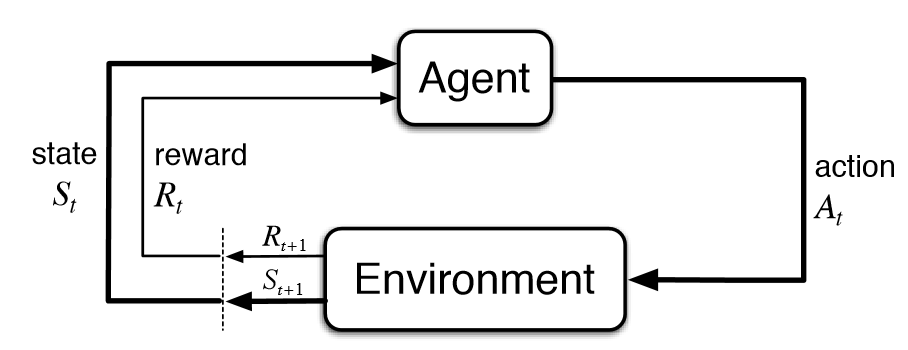
\includegraphics[scale=0.7]{Chapter1/img/RL.png}
\caption{Reinforcement Learning}
\label{fig:rl}
\end{figure}

%To express an RL problem more formally, we have to define the idea of Markov Decision Process (MDP) which consists of states, actions, transition probabilities and rewards which in turn helps in deciding the strategy to be followed by the agent. 

%An MDP consists of states
